
%(BEGIN_QUESTION)
% Copyright 2006, Tony R. Kuphaldt, released under the Creative Commons Attribution License (v 1.0)
% This means you may do almost anything with this work of mine, so long as you give me proper credit

Explain how a vertical height of liquid is able to create pressure, such as in this example:

$$\includegraphics[width=15.5cm]{i00749x01.eps}$$

The deeper you descend into the water, the more pressure there is.

\vskip 10pt

Recall that pressure is defined as force divided by area:

$$P = {F \over A}$$

Calculate the total weight of the water contained in this swimming pool (assuming the pool is circular in shape, the 20-foot dimension being its {\it diameter}), and use this figure to calculate pressure at the bottom of the pool, knowing that pressure is defined as force exerted over an area.  Remember that the density of water is 62.428 lb/ft$^{3}$.

\vskip 10pt

Weight of water = \underbar{\hskip 50pt} lbs

\vskip 10pt

Pressure at bottom of pool = \underbar{\hskip 50pt} PSI

\vskip 10pt

\underbar{file i00749}
%(END_QUESTION)





%(BEGIN_ANSWER)

Weight of water = \underbar{117,674} lbs

\vskip 10pt

Area of circular pool bottom = 45,239 in$^{2}$

\vskip 10pt

Pressure at bottom of pool = $P$ = 2.601 lb/in$^{2}$ (PSI) = 72 inches of water column (" W.C.)

\vskip 10pt


%(END_ANSWER)





%(BEGIN_NOTES)


%INDEX% Physics, static fluids: hydrostatic pressure

%(END_NOTES)


